% Additive recovery from the Witt v4--v7 owners and their original tables.
% Full provenance is retained in the editorial map.
\subsection{Three regional stars and the polarization of their completions}
\label{star27:comparacion}

The preceding incidence construction compares the regions through one
operation. The regional words arise from APP--TRIT--TPK emission;
their encoding by \(\gamma_{A_W}(w)=(w,wA_W)\) retains a support
on the twelve positions. The register \(K\) and the pre-carry
cochain add two readings of the same state: position relative to
the \(729+271\) boundary and the orientation of borrowing.
The following comparison assembles these previously constructed
data while retaining their causal order.

The conserved tables also use an equivalent presentation. With
\(D=\operatorname{diag}(1,-1,-1,-1,-1,-1)\) over
\(\mathbb F_3\), their matrix is \(A_{\rm hist}=A_WD\), and
\[
\gamma_{A_{\rm hist}}(w)=\gamma_{A_W}(w)(I_6\oplus D).
\]
This change multiplies coordinates by units and preserves every
support. The star tables therefore transfer in full to the
presentation \(A_W\) used here.

Write
\[
\begin{aligned}
w_\pi&=010211,&w_e&=201101,&
w_\varphi&=121200,&w_{\rm APP}&=022020,\\
P_\pi&=\{2,4,5,6,7,8,9,10,11\},&
H_e&=\{1,3,4,6,9,10\},\\
H_\varphi&=\{1,2,3,4,7,9\},&
H_{\rm APP}&=\{2,3,5,10,11,12\}.
\end{aligned}
\]
The four sets in the second and third lines are the supports of
the corresponding encoded words. The cochain
\[
s=(7,297,353,-430,-715,-1199,-3,286,-894,-528,380,663)
\]
determines the partition
\[
H^-_\alpha=\{4,5,6,7,9,10\},\qquad
H^+_\alpha=\{1,2,3,8,11,12\}.
\]
The signs are thus fixed before decimal normalization. For a
four-subset \(B\), denote the matching of its star by
\[
\mu_W(B)=\{H\setminus B:H\in\mathcal H,\ B\subset H\}.
\]
A pair has type \(++\), \(--\), or \(+-\) according as it
contains zero, two, or one point of \(H^-_\alpha\).
Its signature is
\(\nu(B)=(n_{++}(B),n_{--}(B),n_{+-}(B))\).

\begin{proposition}[Comparison of the three regional intersections]
\label{star27:tres}
The four-subsets
\[
B_K=H_e\cap P_\pi,\qquad
B_\varphi=H_\varphi\cap P_\pi,\qquad
B_{\rm APP}=H_{\rm APP}\cap P_\pi
\]
have the twelve completions and signatures listed in
Table~\ref{star27:tabla-tres}.
\end{proposition}

\begin{table}[htbp]
\centering\small
\begin{tabular}{lll}
\toprule
Four-subset and signature & Added pair & Resulting hexad\\
\midrule
\(B_K=\{4,6,9,10\}\) & \(\{1,3\}_{++}\) & \(\{1,3,4,6,9,10\}\)\\
\(\nu(B_K)=(3,1,0)\) & \(\{2,11\}_{++}\) & \(\{2,4,6,9,10,11\}\)\\
 & \(\{5,7\}_{--}\) & \(\{4,5,6,7,9,10\}\)\\
 & \(\{8,12\}_{++}\) & \(\{4,6,8,9,10,12\}\)\\
\midrule
\(B_\varphi=\{2,4,7,9\}\) & \(\{1,3\}_{++}\) & \(\{1,2,3,4,7,9\}\)\\
\(\nu(B_\varphi)=(1,0,3)\) & \(\{5,11\}_{+-}\) & \(\{2,4,5,7,9,11\}\)\\
 & \(\{6,12\}_{+-}\) & \(\{2,4,6,7,9,12\}\)\\
 & \(\{8,10\}_{+-}\) & \(\{2,4,7,8,9,10\}\)\\
\midrule
\(B_{\rm APP}=\{2,5,10,11\}\) & \(\{1,4\}_{+-}\) & \(\{1,2,4,5,10,11\}\)\\
\(\nu(B_{\rm APP})=(1,1,2)\) & \(\{3,12\}_{++}\) & \(\{2,3,5,10,11,12\}\)\\
 & \(\{6,7\}_{--}\) & \(\{2,5,6,7,10,11\}\)\\
 & \(\{8,9\}_{+-}\) & \(\{2,5,8,9,10,11\}\)\\
\bottomrule
\end{tabular}
\caption{The three stars with the same reference polarization.
Each row retains the four-subset, complementary pair, and complete hexad.}
\label{star27:tabla-tres}
\end{table}

\begin{proof}
Applying \(\gamma_{A_W}\) to the four regional words yields
the stated supports. For each four-subset, enumerate the hexads
of \(\mathcal H\) that contain it. The relation \(\lambda_4=4\)
ensures that the four completions in the table exhaust the star.
Finally, intersection of each pair with \(H^-_\alpha\)
determines its sign. Every operation takes place within the
finite design already constructed.
\end{proof}

The three signatures distinguish concrete incidence roles.
The star of \(B_K\) separates three positive pairs and one
negative pair; that of \(B_\varphi\) contains three mixed pairs;
that of \(B_{\rm APP}\) combines all three classes. The
distinction persists even when two stars share the pair
\(\{1,3\}\).

\begin{figure}[htbp]
\centering
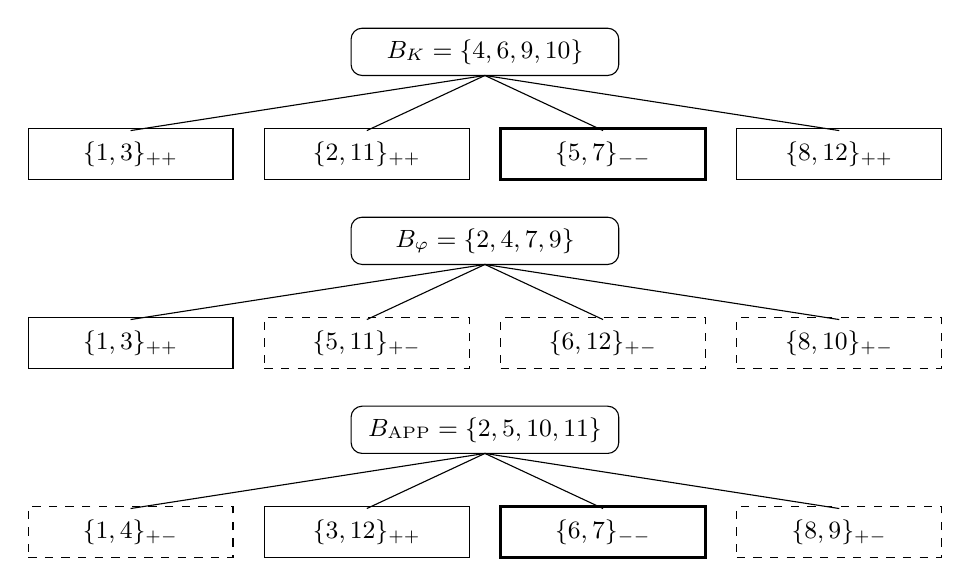
\begin{tikzpicture}[x=1cm,y=1cm,every node/.style={font=\small},
 core/.style={draw,rounded corners,minimum width=3.4cm,minimum height=.6cm},
 petal/.style={draw,minimum width=2.6cm,minimum height=.65cm}]
\foreach \y/\name in {0/{B_K=\{4,6,9,10\}},
 -2.4/{B_\varphi=\{2,4,7,9\}},-4.8/{B_{\rm APP}=\{2,5,10,11\}}}
 {\node[core] at (0,\y) {\(\name\)};
  \foreach \x in {-4.5,-1.5,1.5,4.5}
    {\draw (0,\y-.3)--(\x,\y-1);}}
\node[petal] at (-4.5,-1.3) {\(\{1,3\}_{++}\)};
\node[petal] at (-1.5,-1.3) {\(\{2,11\}_{++}\)};
\node[petal,very thick] at (1.5,-1.3) {\(\{5,7\}_{--}\)};
\node[petal] at (4.5,-1.3) {\(\{8,12\}_{++}\)};
\node[petal] at (-4.5,-3.7) {\(\{1,3\}_{++}\)};
\node[petal,dashed] at (-1.5,-3.7) {\(\{5,11\}_{+-}\)};
\node[petal,dashed] at (1.5,-3.7) {\(\{6,12\}_{+-}\)};
\node[petal,dashed] at (4.5,-3.7) {\(\{8,10\}_{+-}\)};
\node[petal,dashed] at (-4.5,-6.1) {\(\{1,4\}_{+-}\)};
\node[petal] at (-1.5,-6.1) {\(\{3,12\}_{++}\)};
\node[petal,very thick] at (1.5,-6.1) {\(\{6,7\}_{--}\)};
\node[petal,dashed] at (4.5,-6.1) {\(\{8,9\}_{+-}\)};
\end{tikzpicture}
\caption{Comparison of the three stars. Each connection represents
the union of the upper four-subset with one pair; the twelve complete
hexads appear in Table~\ref{star27:tabla-tres}. Thick outlines
indicate negative pairs and dashed outlines mixed pairs.
The connections represent incidence.}
\label{star27:figura}
\end{figure}

\begin{proposition}[Coupling of corona, incidence, and sign]
\label{star27:acoplamiento}
For the previously constructed dodecaphasic register,
\[
B_K=\{i:K_i\geq729\}=H_e\cap P_\pi=\{4,6,9,10\}.
\]
The unique hexad \(H\in\mathcal H\) satisfying
\(H\cap P_\pi=B_K\) is \(H_e\). Moreover,
\[
H^-_\alpha=B_K\sqcup\{5,7\},\qquad
(B_\varphi\setminus B_K)\cap H^-_\alpha=\{7\}.
\]
\end{proposition}

\begin{proof}
The register
\(K=(234,543,140,729,659,824,621,58,914,794,146,601)\)
reaches or exceeds \(729\) at precisely the four stated
positions. Comparison with the supports proves the first
equality. A hexad with intersection \(B_K\) belongs to
the star of \(B_K\); among its four pairs, only
\(\{1,3\}\) is disjoint from \(P_\pi\). This proves
the relative uniqueness of \(H_e\). The table identifies
the negative pair \(\{5,7\}\). Finally,
\(B_\varphi\setminus B_K=\{2,7\}\), and the signs
\(s_2=297>0\), \(s_7=-3<0\) determine the pivot \(7\).
\end{proof}

The four-subset, sign, and normalization retain distinct roles.
Incidence fixes the completion \(H^-_\alpha\); the Archimedean
lift of the complete cochain also uses the magnitudes, positional
order, and carries already established in the closure of
\(\alpha\). This composition explains how one genealogy
produces both a geometric boundary reading and a numerical reading.

\subsection{Polarized classification of the 495 four-subsets}
\label{star27:clasificacion}

\begin{theorem}[Signature census and regional restriction]
\label{star27:censo}
The \(495=\binom{12}{4}\) four-subsets are distributed as
in Table~\ref{star27:tabla-censo}. The last column counts
hexads \(H\) with \(|H\cap P_\pi|=4\), classified by
\(\nu(H\cap P_\pi)\).
\end{theorem}

\begin{table}[htbp]
\centering
\begin{tabular}{ccc}
\toprule
\(\nu=(n_{++},n_{--},n_{+-})\)&Four-subsets&Regional hexads\\
\midrule
\((3,1,0)\)&15&9\\
\((1,3,0)\)&15&0\\
\((2,2,0)\)&45&9\\
\((1,1,2)\)&180&18\\
\((1,0,3)\)&120&18\\
\((0,1,3)\)&120&0\\
\midrule
Total&495&54\\
\bottomrule
\end{tabular}
\caption{Complete classification and restriction to the support
\(P_\pi\). The two columns count different objects: four-subsets
and hexads.}
\label{star27:tabla-censo}
\end{table}

\begin{proof}
The following procedure is an exact enumeration of the finite
domain. Form the \(3^6\) words \(w\), compute \((w,wA_W)\)
modulo \(3\), and retain their weight-six supports without
repetition. This gives \(\mathcal H\), with \(132\) elements.
For each \(B\in\binom{[12]}4\), form \(\mu_W(B)\), count
the intersections of its four pairs with \(H^-_\alpha\),
and increment the entry for the resulting signature. The six
counts are \(15,15,45,180,120,120\). They sum to \(495\),
and each four-subset is processed once. For the last column,
traverse the \(132\) hexads, retain the \(54\) whose
intersection has size four, and apply the same function
\(\nu\) to that intersection. The operations are set
comparisons and arithmetic in \(\mathbb F_3\); the
reproducible certificate retains the complete input--output table.
\end{proof}

The signature \((3,1,0)\) occurs for fifteen four-subsets.
The regional frame is characterized jointly by the corona of
\(K\), the intersection \(H_e\cap P_\pi\), and the cochain
sign, as established in Proposition~\ref{star27:acoplamiento}.

\subsection{Rigidity of the ordered four-support frame}
\label{star27:rigidez}

Let \(G_W=\langle\sigma_B:|B|=4\rangle\), already computed
in Proposition~\ref{exc:m12}. For an ordered collection of
supports, define
\[
\operatorname{Stab}_{G_W}(S_1,\ldots,S_r)
=\{g\in G_W:g(S_j)=S_j\ \text{for every }j\}.
\]
Each support is preserved individually; internal permutations
of its points remain permitted.

\begin{theorem}[Joint rigidity of the four incidences]
\label{star27:marco}
The stabilizers have the following orders:
\[
\begin{array}{l|r}
\text{preserved data}&\text{order}\\ \hline
H^-_\alpha&720\\
H^-_\alpha,\ 6&120\\
B_K&192\\
B_K,H^-_\alpha&48\\
B_K,H^-_\alpha,H_e&16\\
H^-_\alpha,H_e,H_\varphi&2\\
H^-_\alpha,H_e,H_\varphi,H_{\rm APP}&1
\end{array}
\]
The second row also preserves the point \(6\).
In particular,
\[
\operatorname{Stab}_{G_W}
(H^-_\alpha,H_e,H_\varphi,H_{\rm APP})=\{\operatorname{id}\}.
\]
\end{theorem}

\begin{proof}
Use the closure under composition of the six explicit
permutations in Proposition~\ref{exc:m12}. On its \(95040\)
elements evaluate the predicates \(g(S_j)=S_j\), together
with \(g(6)=6\) where required. Summing their indicators
gives \(720,120,192,48,16,2,1\), respectively. The identity
satisfies every condition; the last cardinality proves
that it is the unique element. The closure algorithm
terminates when the set stabilizes, and the stabilizer
filters are then applied to the complete group.
\end{proof}

The table compares seven marked configurations. Two useful
inclusion chains are those determined by
\((B_K)\), \((B_K,H^-_\alpha)\),
\((B_K,H^-_\alpha,H_e)\), and by
\((H^-_\alpha)\), \((H^-_\alpha,H_e,H_\varphi)\),
\((H^-_\alpha,H_e,H_\varphi,H_{\rm APP})\).
Final rigidity means that the ordered regional frame fixes
all residual freedom within \(G_W\). Its domain is the
action on twelve positions; subsequent transport to
lattices and algebras retains the maps belonging to
those realizations.

\subsection{Finite incidence topology and preservation of its domain}
\label{star27:topologia}

The simplicial complex generated by the \(132\) hexads
has face vector
\[
(f_0,f_1,f_2,f_3,f_4,f_5)=(12,66,220,495,792,132)
\]
and Euler characteristic
\(\chi=12-66+220-495+792-132=331\).
Indeed, each five-subset has a unique hexadic extension;
every smaller subset belongs to one of these five-subsets,
and the maximal faces are the hexads.

The bipartite graph between four-subsets and hexads has
\[
|V|=495+132=627,\qquad |E|=495\cdot4=132\cdot15=1980.
\]
It is connected. Let \(H,H_*\) be distinct hexads; their
intersection has at most four points because each five-subset
has a unique extension. Choose a four-subset \(B\subset H\)
containing \(H\cap H_*\), and a point \(p\in H_*\setminus H\).
The unique extension \(H'\) of \(B\cup\{p\}\) is joined to
\(H\) by the bipartite path \(H-B-H'\) and satisfies
\(|H'\cap H_*|>|H\cap H_*|\). Repeating the operation
reaches \(H_*\); containing five of its points already
forces equality. Every four-subset is incident to four
hexads, so it too belongs to this single component.
Its first Betti number is therefore
\[
\beta_1=|E|-|V|+1=1354.
\]
An exhaustive traversal also verifies connectedness.
For unordered pairs of distinct hexads, the intersection
census is
\[
\begin{array}{c|rrrr}
|H\cap H'|&0&2&3&4\\ \hline
\#\{H,H'\}&66&2970&2640&2970 .
\end{array}
\]
The sum \(8646=\binom{132}{2}\) covers every pair.

These invariants describe the complex and its incidence graph.
The junction micrograph \(U_6=A|B\) separately retains its
\(96\) vertices, \(234\) edges, six components, and
\(\beta_1=234-96+6=144\). Likewise, compositions of the
\(\sigma_B\) act on incidence positions, whereas
\(\Gamma_9\) transports the TPK state with memory.
This distinction relates the readings through their
effective maps and preserves, at each level, the data
used by the operation.
